\documentclass{beamer}
\usepackage{xeCJK}
\usepackage{graphicx}
\usepackage{xcolor}
\usepackage{setspace}

% ============= setup =============
\setCJKmainfont{Taipei Sans TC Beta}
\setCJKsansfont{Taipei Sans TC Beta}
\setmainfont{Taipei Sans TC Beta}
\hypersetup{
    colorlinks=true,
    linkcolor=black,
    urlcolor=blue
}
\renewcommand{\baselinestretch}{1.25}
\usetheme{Madrid}
\usecolortheme{crane}
\setbeamertemplate{items}[circle]
\setbeamertemplate{section in toc}{\inserttocsectionnumber.~\inserttocsection}
\AtBeginSection[]{
    \begin{frame}
        \vfill
        \centering
        \begin{beamercolorbox}[sep=8pt,center,shadow=true,rounded=true]{title}
            \usebeamerfont{title}\insertsectionhead\par%
        \end{beamercolorbox}
        \vfill
    \end{frame}
}

\title{枚舉}
\author{temmie}
\date{}
% ============= setup =============

\begin{document}

\begin{frame}
    \titlepage
\end{frame}

\begin{frame}
    \tableofcontents
\end{frame}

\section{枚舉介紹}

\begin{frame}
    \frametitle{枚舉的定義}
    \begin{itemize}
        \item 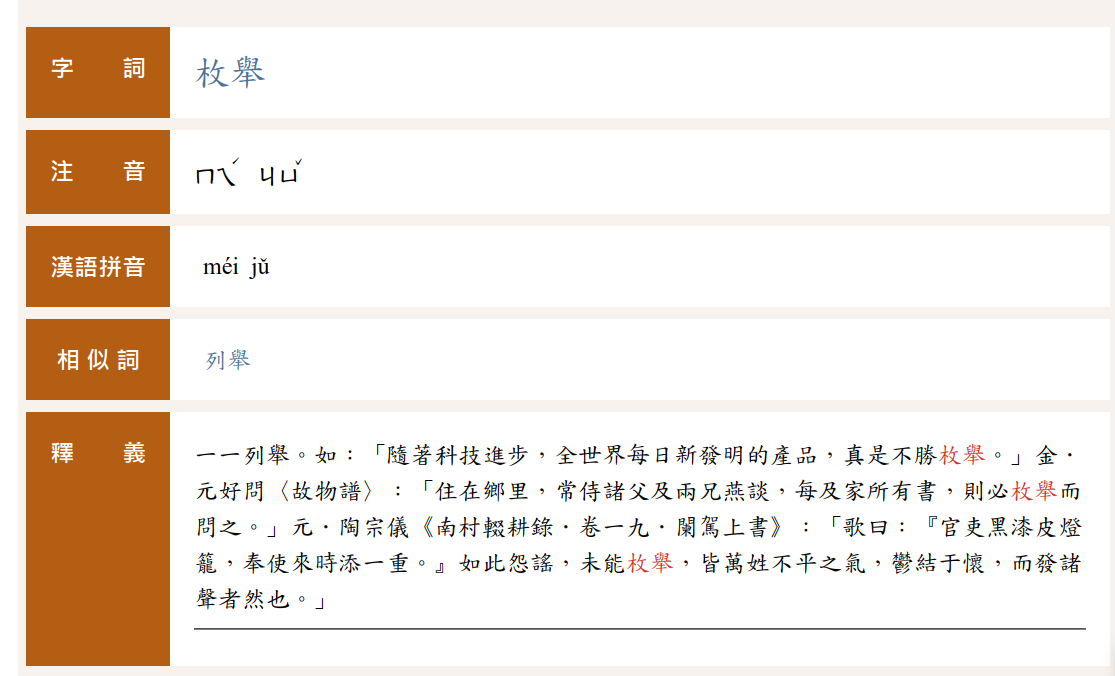
\includegraphics[width=9.0cm]{img/img_1.png}
        \item 只要把所有需要的情況列出來,然後找哪個是答案
    \end{itemize}
\end{frame}

\begin{frame}
    \frametitle{枚舉的用處}
    \begin{itemize}
        \item 我們之前有提過高中的比賽都會有部份分數
        \item 在大部份的比賽裡都會有關於枚舉的子任務
        \item 通常這些題目不會特別卡枚舉,撈分可說是非常好用
        \item \textbf{\textcolor{red}{我認為這是所有單元裡面 CP 值最高的}}
    \end{itemize}
\end{frame}

\section{全部枚舉}

\begin{frame}
    \frametitle{枚舉的方式}
    \begin{itemize}
        \item 把題目給予的所有情況都列出一遍,即可得到答案
        \item 通常會有三種方式:迴圈枚舉、全排列枚舉、位元枚舉、遞迴枚舉
    \end{itemize}
\end{frame}

\section{迴圈枚舉}

\begin{frame}
    \frametitle{例題}
    \begin{block}{迴圈枚舉}
        \href{https://atcoder.jp/contests/abc144/tasks/abc144_b}{題目連結}\\
        給你一個正整數 $N$,請判斷它是不是兩個 $1 \sim 9$ 的數的積\\
        保證 $1 \leq N \leq 100$
    \end{block}
\end{frame}

\begin{frame}
    \frametitle{迴圈枚舉}
    \begin{itemize}
        \item 如果一個題目的參數較少,則可以用 for 迴圈枚舉所有參數
        \item 另外要注意時間複雜度的限制
    \end{itemize}
\end{frame}

\section{全排列枚舉}

\begin{frame}
    \frametitle{例題}
    \begin{block}{全排列枚舉}
        \href{https://cses.fi/problemset/task/1622}{題目連結}\\
        給你一個字串 $S$,請從從小到大的字典序輸出所有不同排列\\
        保證 $1 \leq |S| \leq 8$
    \end{block}
\end{frame}

\begin{frame}
    \frametitle{全排列枚舉}
    \begin{itemize}
        \item 這時候需要用到一個特殊的語法  next\_permutation(\textcolor{red}{L}, \textcolor{red}{R})
        \item 他會把 [ L, R ) 範圍內的替換成下一個字典序的排列
        \item 並且會回傳是否排列成功
        \vspace{0.5cm}
        \item<2-> 要做到「全排列」這件事情,其實只需要從最小字典序的排列\\
        不斷執行直到 next\_permutation 不能排列為止
        \item<2-> 時間複雜度為 $O(n!)$,大概可以接受到 $n \leq 10$
    \end{itemize}
\end{frame}

\begin{frame}
    \frametitle{全排列枚舉模板}
    \begin{itemize}
        \item 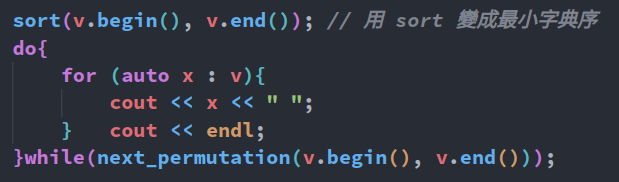
\includegraphics[width=10.0cm]{img/img_2.png}
        \item 這裡出現了一個新的語法 do...while
        \item 和 while 的概念一模一樣,不過是等到裡面的東西執行完再判斷
        \item 這裡需要使用的原因是因為我們也要判斷第一個排列是否為答案
    \end{itemize}
\end{frame}

\begin{frame}
    \frametitle{例題}
    \begin{block}{全排列枚舉}
        \href{https://cses.fi/problemset/task/1623}{題目連結}\\
        給你 $n$ 個蘋果,每個重量為 $p_i$,請問該怎麼分成兩組讓它們重量差最小\\
        保證 $1 \leq n \leq 20$ 且 $1 \leq p_i \leq 10^9$
    \end{block}
\end{frame}

\begin{frame}
    \frametitle{位元枚舉}
    \begin{itemize}
        \item 位元枚舉通常用在「分成兩組」、「拿或不拿」的問題
        \item 這時候不能使用全排列,有什麼是可以判斷要不要用某個參數呢?
        \vspace{0.5cm}
        \item<2-> 二進位!我們可以使用二進位來分組
        \item<2-> 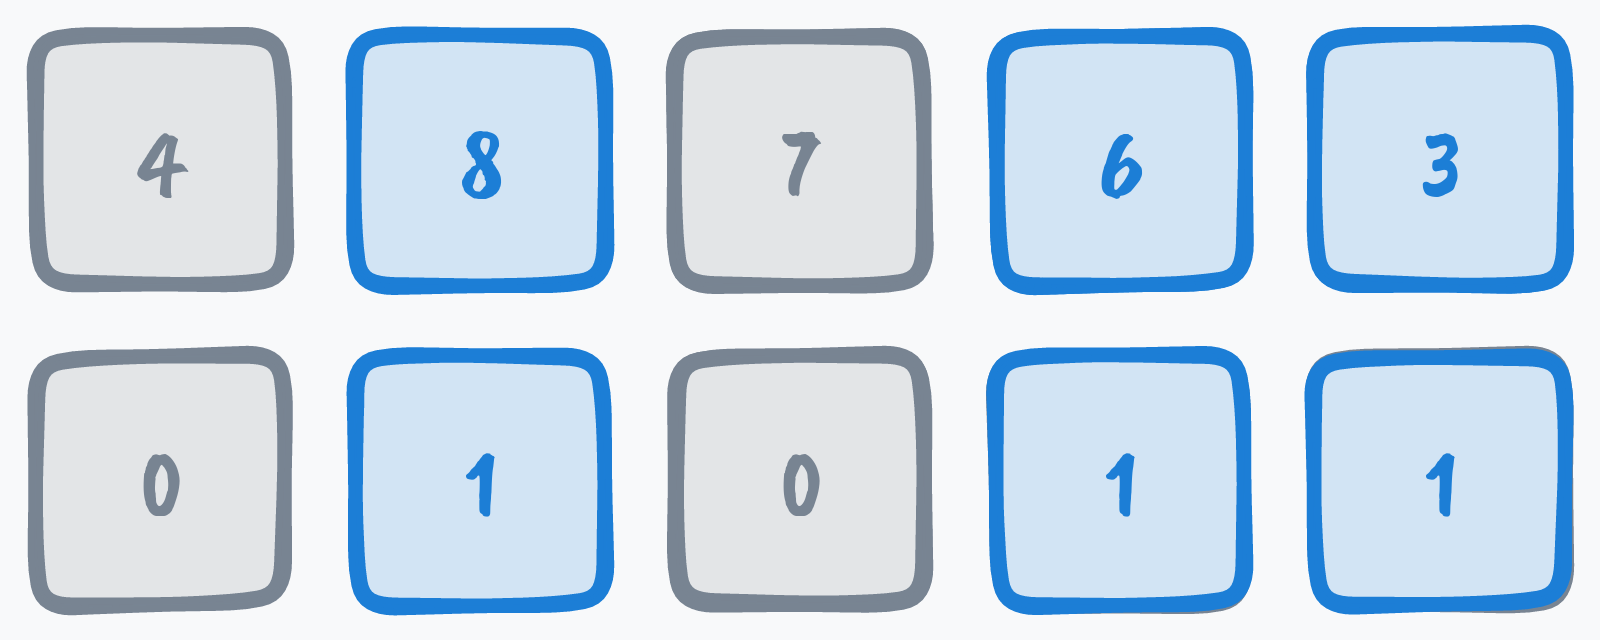
\includegraphics[width=7.0cm]{img/img_3.png}
    \end{itemize}
\end{frame}

\section{位元枚舉}

\begin{frame}
    \frametitle{位元枚舉}
    \begin{itemize}
        \item 由於要枚舉每一個二進位的可能,其實就是枚舉 $0 \sim 2^n-1$!
        \item 原因是因為 $n$ bit可以組成 $0 \sim 2^n-1$ 的所有數字
        \vspace{0.5cm}
        \item 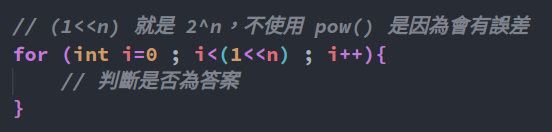
\includegraphics[width=9.0cm]{img/img_4}
    \end{itemize}
\end{frame}

\begin{frame}
    \frametitle{位元枚舉}
    \begin{itemize}
        \item 枚舉完一種排列後,就要分組並且計算答案
    \end{itemize}
\end{frame}

\begin{frame}
    \frametitle{位元枚舉}
    \begin{itemize}
        \item 枚舉完一種排列後,就要檢查是否為答案
        \item 我們可以將 1 不斷的去「掃描」每個位元,並且做 \& 運算
        \item 只要結果不是 0 的話就代表這個為 true,也就是同一組的意思
    \end{itemize}
\end{frame}

\begin{frame}
    \frametitle{位元枚舉}
    \begin{itemize}
        \item 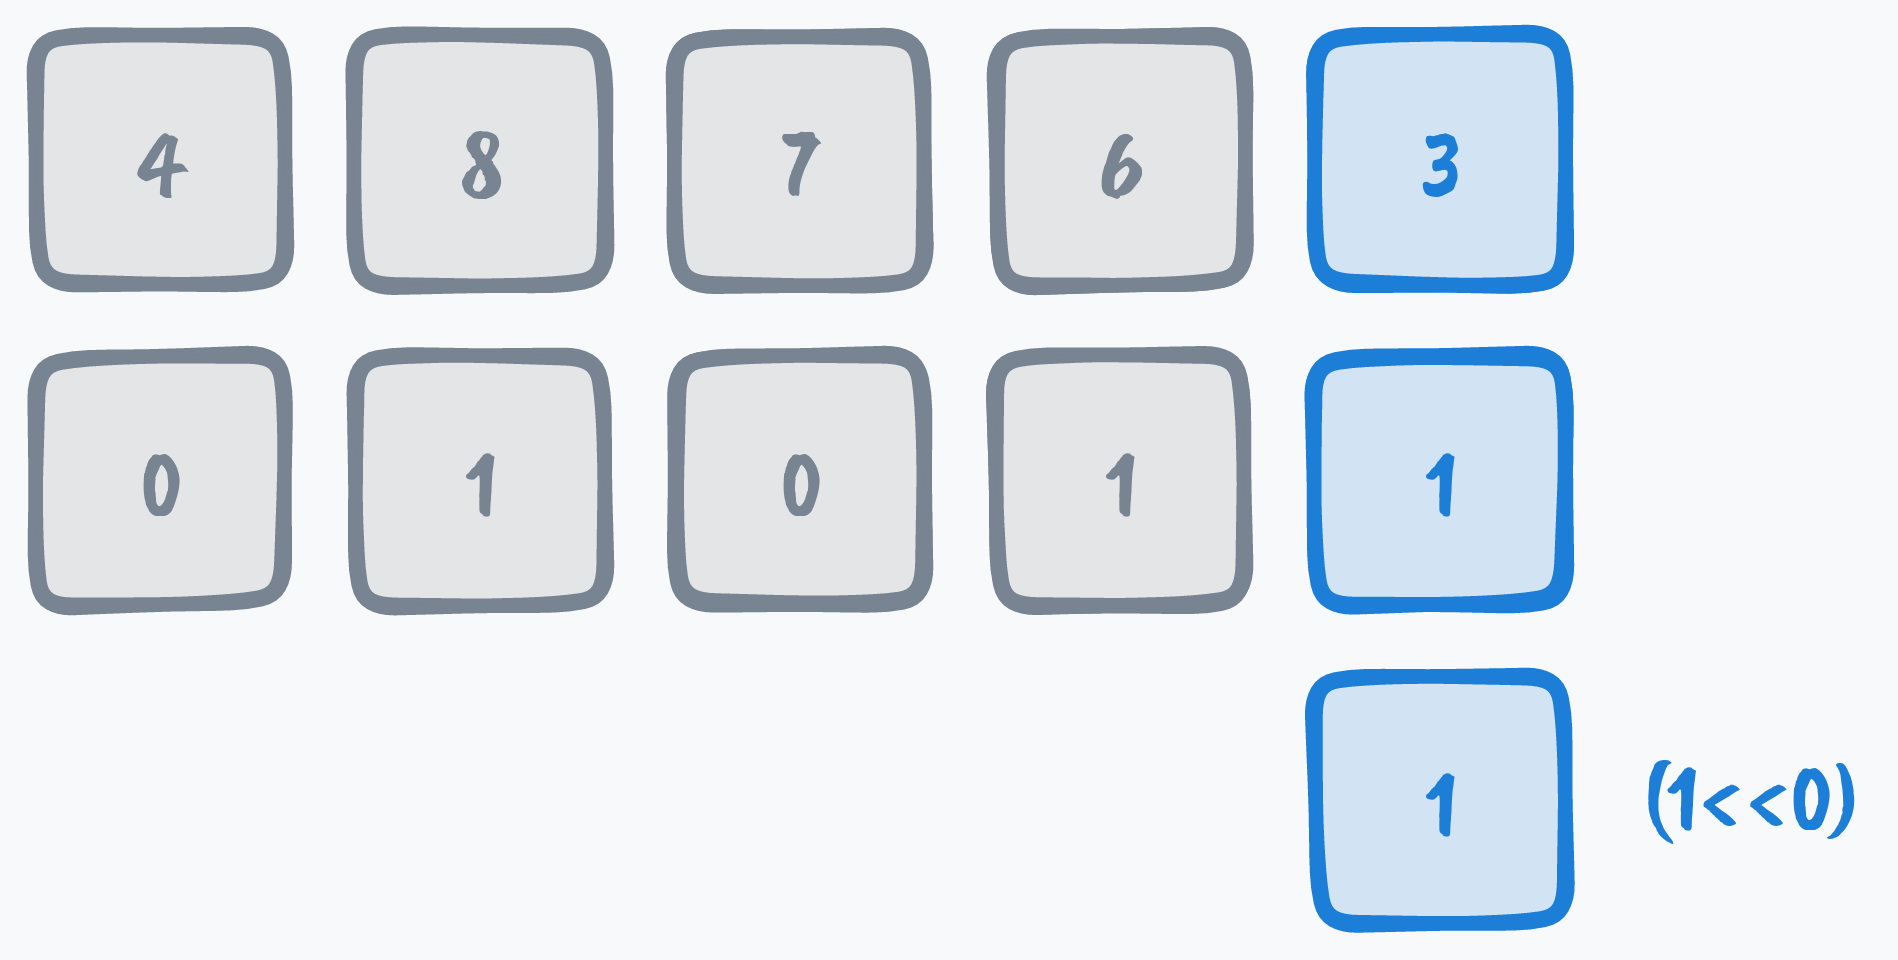
\includegraphics[width=10.0cm]{img/img_5.png}
    \end{itemize}
\end{frame}

\begin{frame}
    \frametitle{位元枚舉}
    \begin{itemize}
        \item 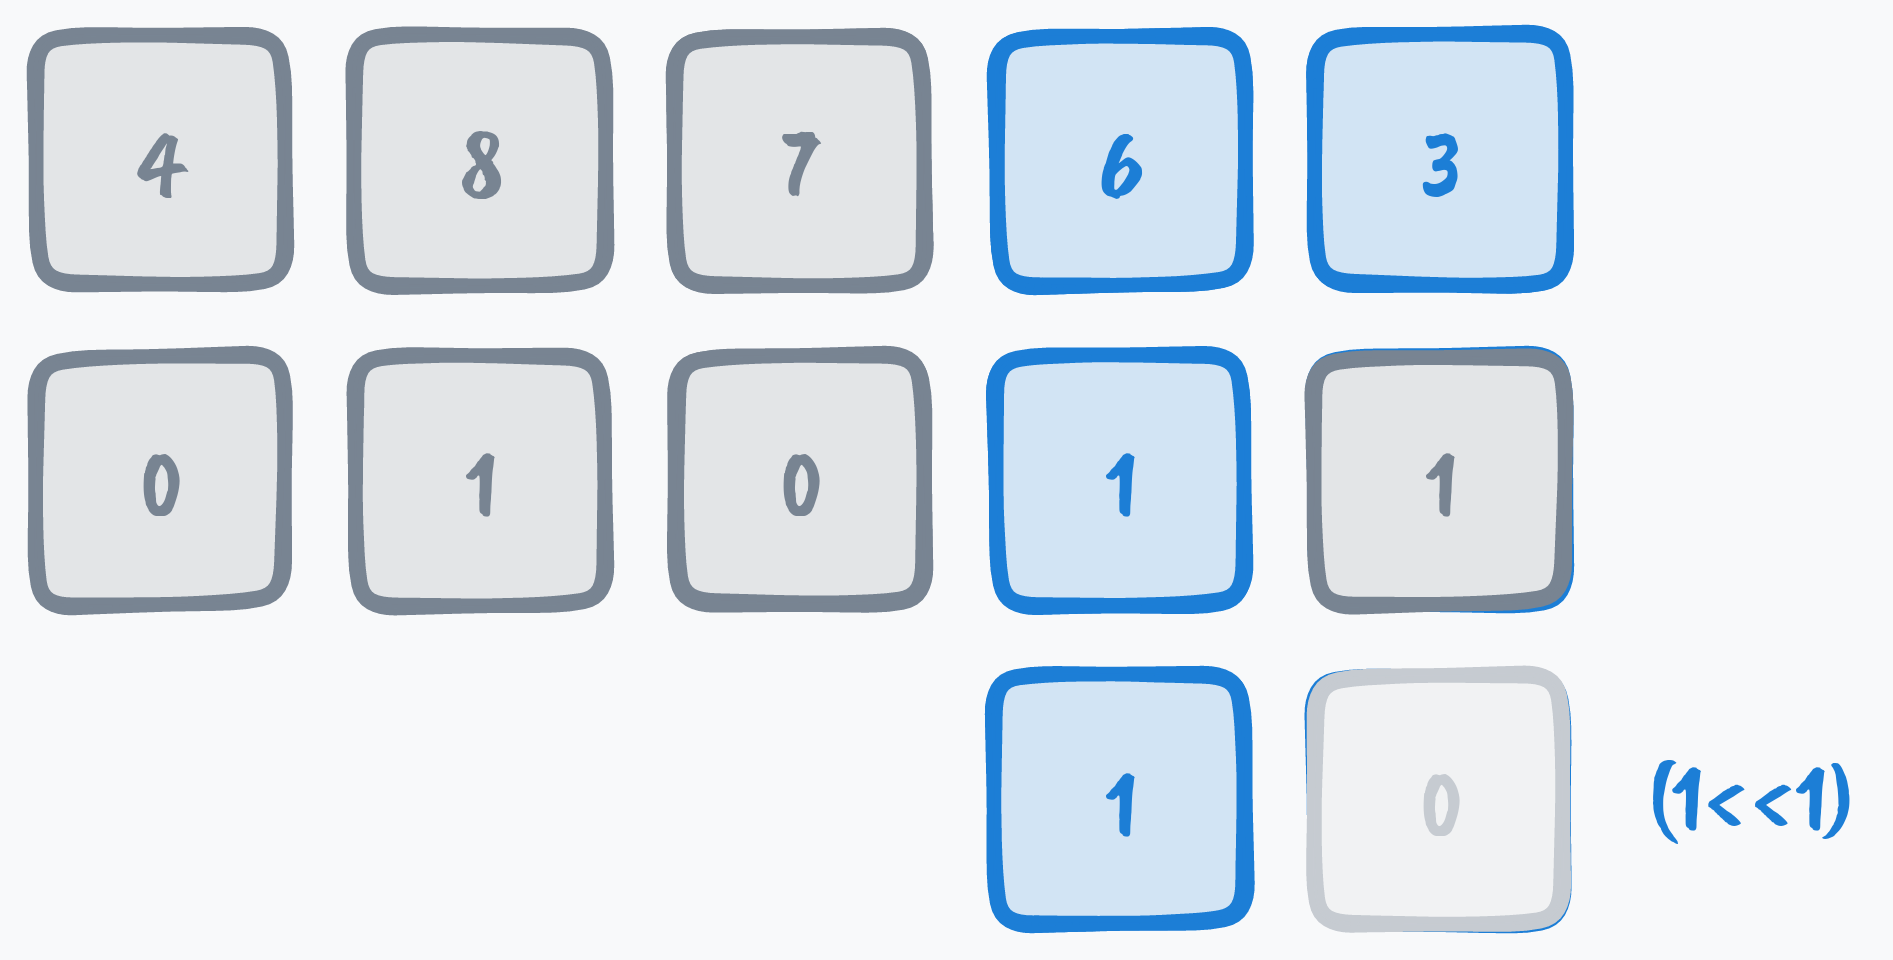
\includegraphics[width=10.0cm]{img/img_6.png}
    \end{itemize}
\end{frame}

\begin{frame}
    \frametitle{位元枚舉}
    \begin{itemize}
        \item 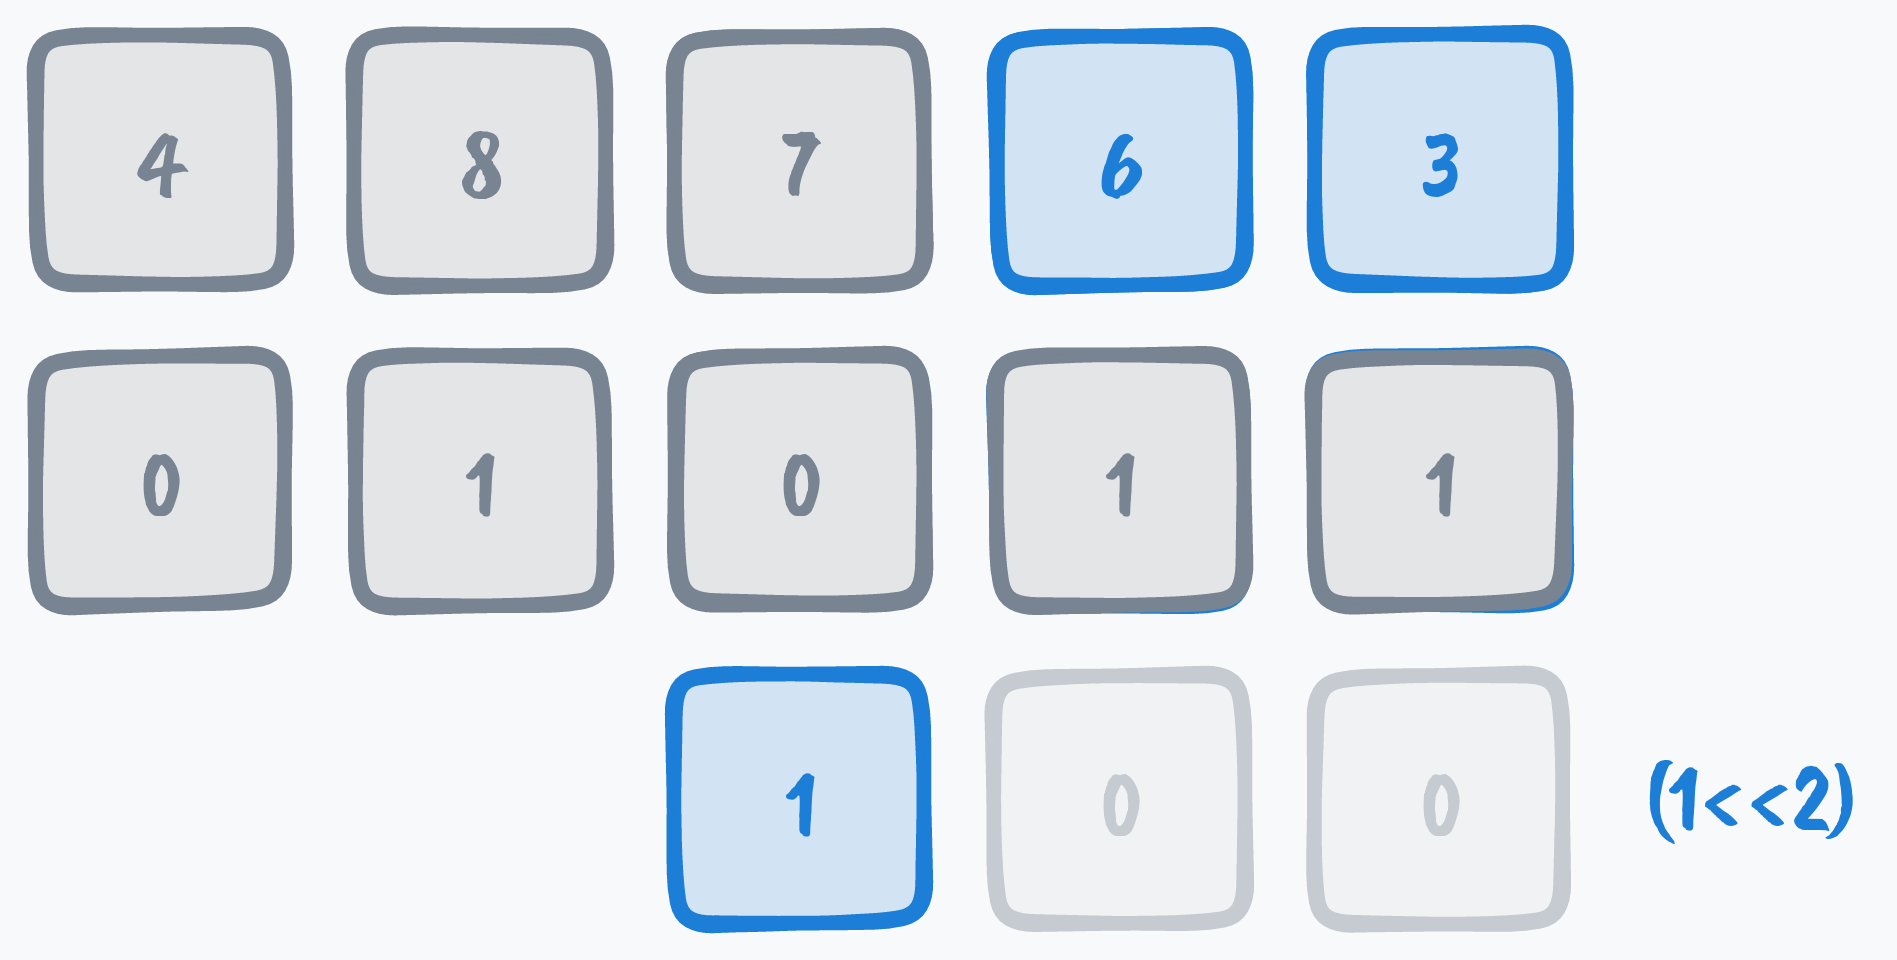
\includegraphics[width=10.0cm]{img/img_7.png}
    \end{itemize}
\end{frame}

\begin{frame}
    \frametitle{位元枚舉}
    \begin{itemize}
        \item 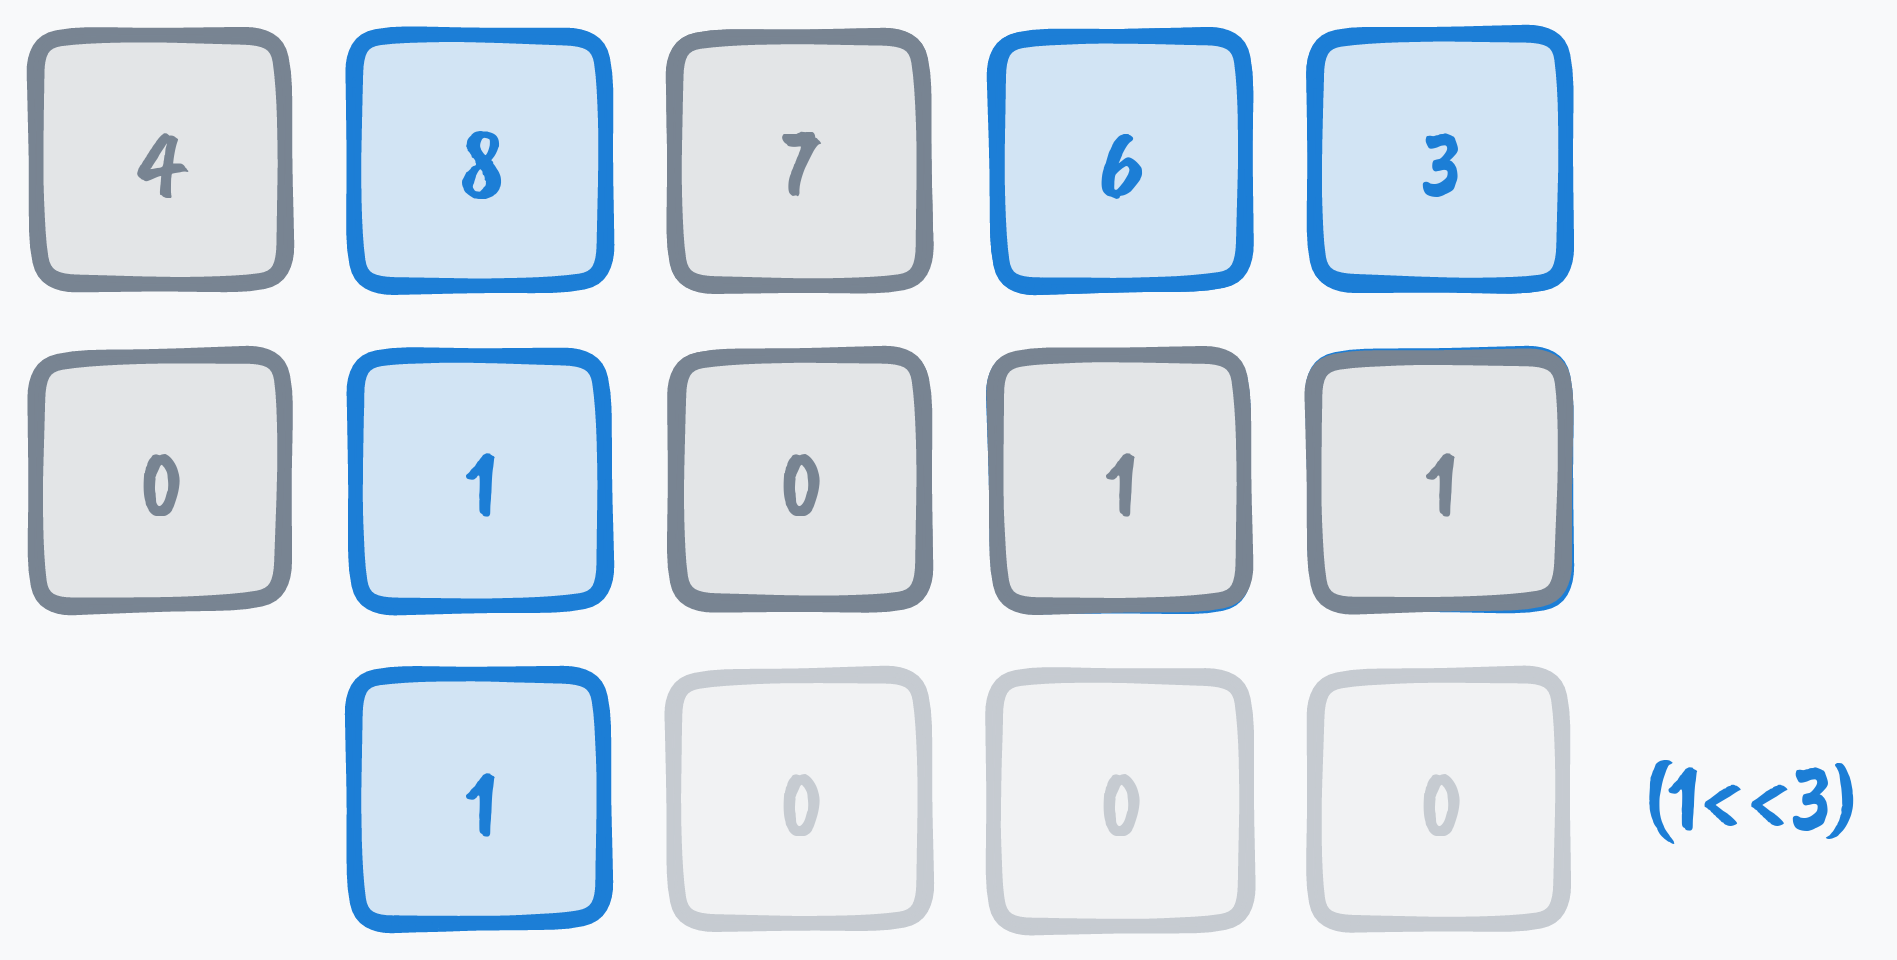
\includegraphics[width=10.0cm]{img/img_8.png}
    \end{itemize}
\end{frame}

\begin{frame}
    \frametitle{位元枚舉}
    \begin{itemize}
        \item 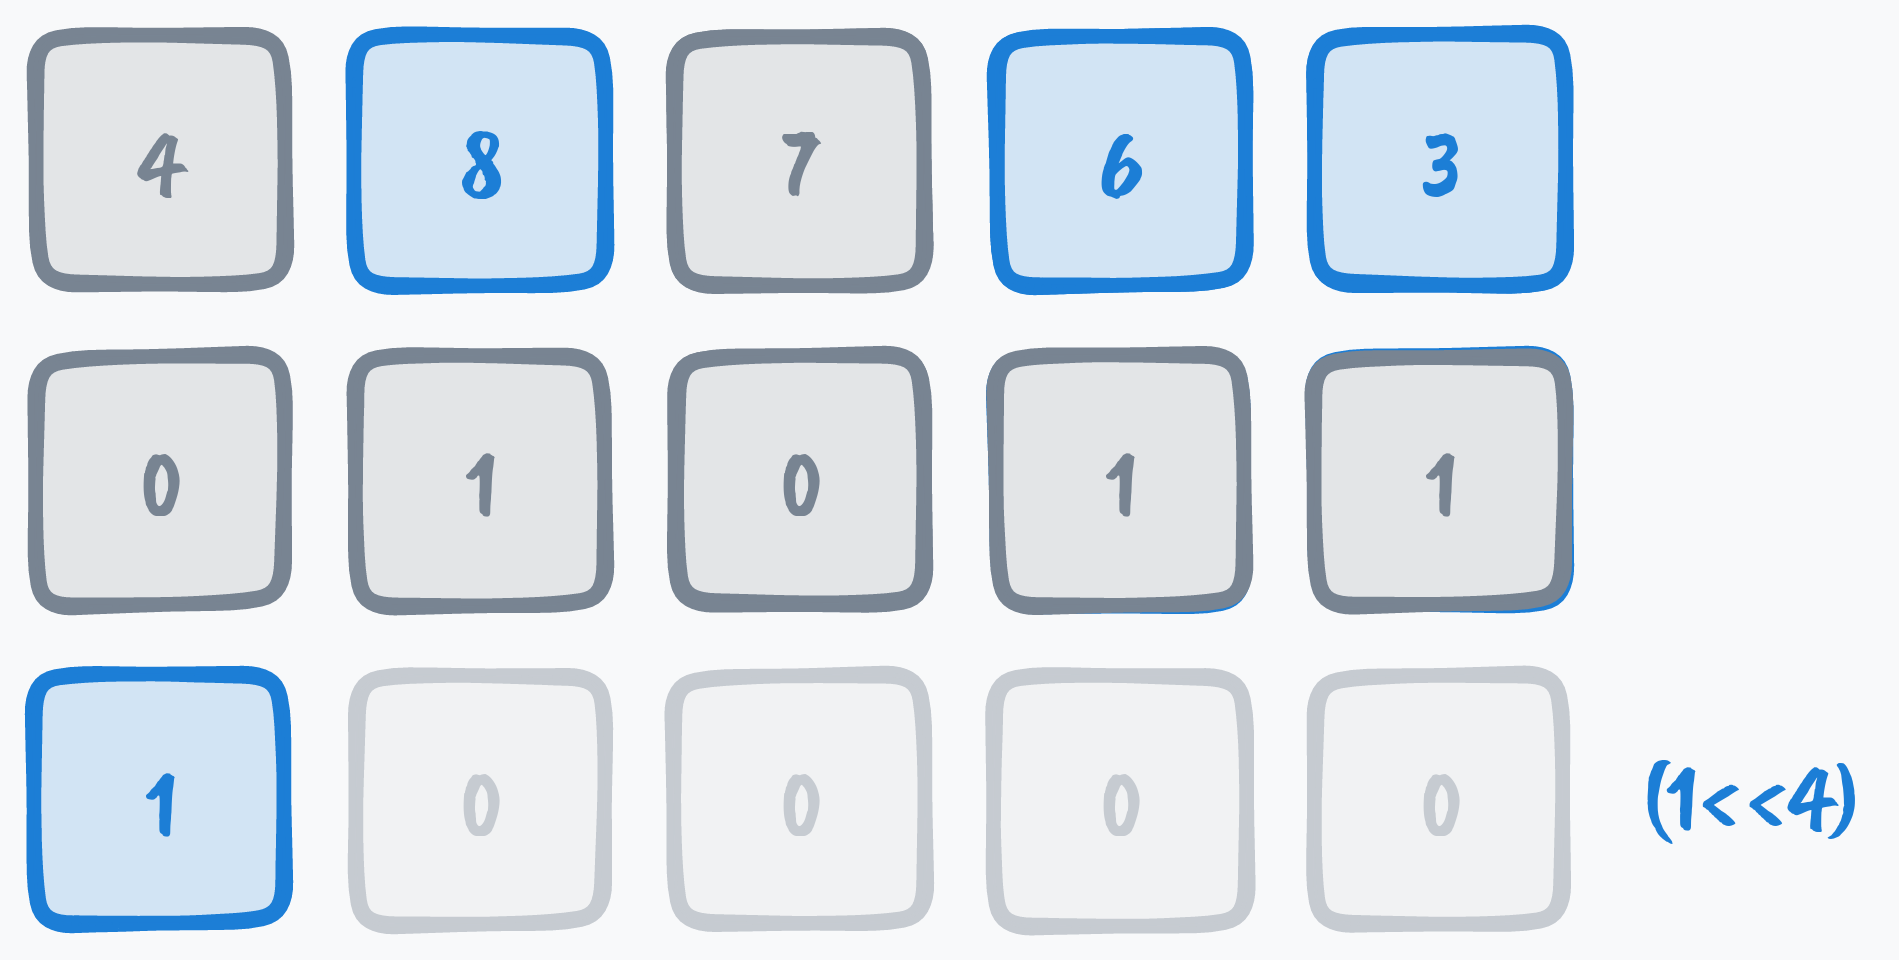
\includegraphics[width=10.0cm]{img/img_9.png}
    \end{itemize}
\end{frame}

\begin{frame}
    \frametitle{位元枚舉}
    \begin{itemize}
        \item 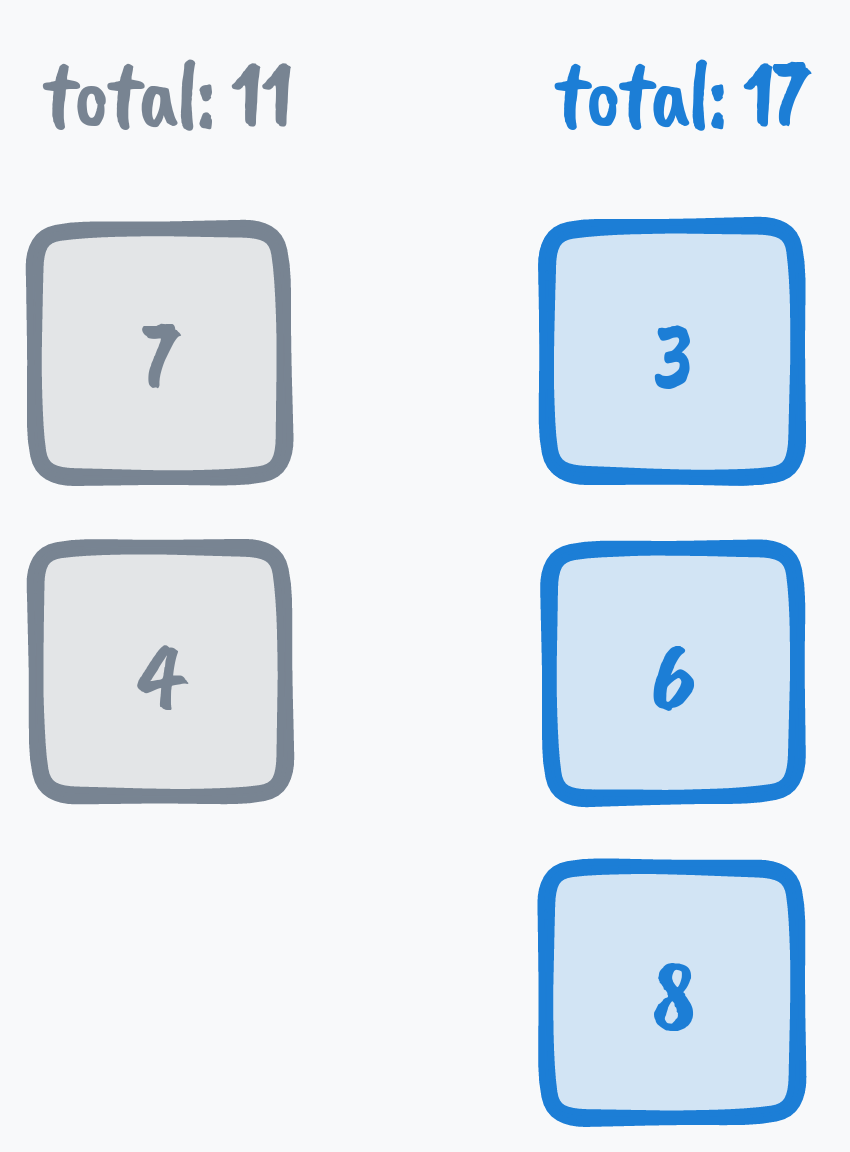
\includegraphics[width=5.0cm]{img/img_10.png}
    \end{itemize}
\end{frame}

\end{document}